\chapter{Reinforcement Learning}

\label{ch:rl}

\section{Reinforcement Learning}

\label{sec:rl}

% Motivation
In this section, we will briefly review the most important aspects of classic
\emph{Reinforcement Learning} (RL)\nomenclature{RL}{Reinforcement Learning}.
These concepts are relevant because they are also found in Deep Reinforcement
Learning (Deep RL), which is a central component of the agent we will design.
Excellent references for these topics are \cite{bib:rl-book},
\cite{bib:probabilistic-rl}, and \cite{bib:ml-book-murphy} for graphical
models.

% Agent-env interface
In AI, we commonly isolate two entities, the agent and the environment, which
continuously interact. At each instant, the agent receives observations from
the environment and it executes actions in response. In RL specifically, the
agent observes the current state of the environment and a numerical reward.
The environment produces high rewards in response to desirable events. The
agent's goal is to maximize the rewards received. The basic setup is
illustrated in Figure~\ref{fig:rl}.

\begin{figure}
	\centering
	\begin{tikzpicture}
		\node [block] (agent) {Agent};
		\node [block, below=of agent] (env) {Environment};
		\draw [flow] ([yshift=2mm]env.west) -- ++(-1.2,0) |-
			([yshift=-2mm]agent.west) node [pos=0.3,right] {reward\\$r$};
		\draw [flow] ([yshift=-2mm]env.west) -- ++(-1.5,0) |-
			([yshift=2mm]agent.west) node [pos=0.3,left] {state\\$s$};
		\draw [flow] (agent.east) -| node [pos=0.7,right] {action\\a}
		($(env.east)+(1.2,0)$) -- (env.east);
	\end{tikzpicture}
	\caption{How agent and environment interact in RL.}
	\label{fig:rl}
\end{figure}


\subsection{Markov Decision Processes}

% MDP
Most RL algorithms assume that the environment dynamics can be modelled with a
\emph{Markov Decision Process} (MDP)\nomenclature{MDP}{Markov Decision
Process}. They do so, because under the independence assumptions taken by MDP,
it's possible to efficiently find the optimal agent's policy.

\begin{definition}
	A Markov Decision Process is a tuple $\langle \stateS, A, T, R, \discount
	\rangle$, where: $\stateS$ is the set of states of the environment; $A$ is
	the action space; $T: \stateS \times A \times \stateS \to \R$ is the
	transition function, which, for ${T(s_{t}, a_{t}, s_{t+1})}$, returns the
	probability $p(s_{t+1} \given s_{t}, a_{t})$ of the transition ${s_{t}
	\xrightarrow{a_{t}} s_{t+1}}$; $R: \stateS \times A \times \stateS \to \R$
	is the reward function; and $\discount \in [0, 1]$ is called ``discount
	factor''\footnote{In this chapter, variables with an integer subscript or
	index refer to the value at the discrete time indicated.}.
\end{definition}

% Markov assumptions
In a RL problem, the functions $T$ and $R$ are unknown. The agent can only
learn them by taking each action and observing the outcomes. Even if they are
unknown, by assuming that they can be modelled with functions ${\stateS \times
A \times \stateS \to \R}$, we introduce some Markov assumptions. In
particular, we assume that the next state of the environment is conditionally
independent on the whole history, given the previous state and action:
$s_{t+1} \perp s_{0}, \dots, s_{t-1} \given s_{t}, a_{t}$. Similarly, the
reward only depends on the last transition of the environment.  Although it's
not required by the model, it is common that rewards are computed just from
desirable configurations of the environment~$s_{t}$, not from specific
transitions $(s_{t-1}, a_{t-1}, s_{t})$. All these assumptions are summarized
in the Directed Graphical Model (DGM)\nomenclature{DGM}{Directed Graphical
Model} of Figure~\ref{fig:mdp}. In a DGM, edges indicate direct conditional
probabilities, while missing arcs indicate conditionally independent
variables.  In Figure~\ref{fig:mdp}, the lack of any arrow between $s_{t-1}$
and $s_{t+1}$ means that future states, hence the rewards, do not depend on
the past history, given the current state~$s_t$.  This is the essence of a
Markov assumption.

\begin{figure}
	\centering
	\begin{tikzpicture}
		\matrix [
			column sep={1cm,between origins}, row sep={1cm,between origins},
		] {
			\&
			\node (am1) [observed node, label=above:$a_{t-1}$] {};
			\& \&
			\node (a) [observed node, label=above:$a_{t}$] {}; \& \\
			\node (stm1) [observed node, label=above:$s_{t-1}$] {};
			\& \&
			\node (st) [observed node, label=above:$s_{t}$] {}; \& \&
			\node (st1) [observed node, label=above:$s_{t+1}$] {}; \\
			\& \&
			\node (r) [observed node, label=below:$r_{t}$] {}; \& \&
			\node (r1) [observed node, label=below:$r_{t+1}$] {}; \\
		};
		\draw (st1) edge [<-] (st) edge [<-] (a);
		\draw [->, dotted] (st) -- (a);
		\draw [->] (st) -- (r);
		\draw [->] (st1) -- (r1);
		\draw (st) edge [<-] (stm1) edge [<-] (am1);
		\draw [->, dotted] (stm1) -- (am1);

		\draw [dashed, gray] (st1) -- +(0.8,0);
		\draw [dashed, gray] (stm1) -- +(-0.8,0);
	\end{tikzpicture}
	\caption{The directed graphical model of an MDP.}
	\label{fig:mdp}
\end{figure}

\begin{example}
	\label{ex:board-games}
	Tic-Tac-Toe, Chess and many other board games can be modelled with an MDP.
	Even games with dice, such as Backgammon. To do so, we define as state
	space~$\stateS$ the set of configurations of the board, and a reward
	function $R(s)$ that returns $1$, if the configuration $s$ is a win, $-1$
	for a loss, and 0 otherwise. Even though most games are deterministic, the
	presence of an opponent makes the transition function~$T$ of the MDP
	nondeterministic.  What these games have in common, is that the player gets
	to see the complete state of the game, which is the current configuration of
	the board. Future states of the game and rewards only depend on the current
	situation, not on the whole play. In Chess, for example, we can determine
	whether a configuration is a win or loss just by looking for a checkmate;
	there is no need to ask the players how the game has been carried out.

	Proving that Markovian $T$ and $R$ exist is easy for board games, because
	the rules of the game define them. As we will see in
	Section~\ref{sec:non-markov}, when $T$ is unknown, as always happens in the
	real-world, it's much more difficult to prove that we're in fact facing an
	MDP.
\end{example}


\subsection{Optimal policies}

The \emph{policy} is the criterion the agent uses to select the actions to
perform. If the environment dynamics can be modelled with an MDP, the
optimal action at time~$t$ only depends on~$s_{t}$. So, there must exist
an optimal policy as $\optimal\policy: \stateS \to A$. However, due to common
estimation errors, it is always better to prefer nondeterministic policies,
which return a probability distribution over the actions. The action at time
$t$ will be sampled according to $a_t \sim \policy(s_t)$. This dependency is
represented by the dotted arrows of Figure~\ref{fig:mdp}. A policy that is a
function only of the state is called ``stationary''.

We will now introduce few basic quantities of RL that serve to define what it
means for an action or a policy to be optimal. The \emph{discounted
return}~$G$ is the combination of all rewards collected:
\begin{equation}
	G \coloneqq r_{0} + \discount\, r_1 + \discount^2 r_2 + \dots =
	\sum_{t=0}^{T} \discount^{t} r_{t}
	\label{eq:return}
\end{equation}
The discount factor, $0 \le \discount \le 1$, decides the relative importance
of immediate and future rewards. Usually, this factor is strictly less than 1
because this stimulates the agent to achieve rewards as soon as possible.
It also produces a finite discounted reward, even for an infinite run, where
$T \to \infty$.  Since the environments we will experiment with are video
games, each play is an episode and the total number of steps in each episode
is finite.

It is now clear, that the optimal policy should always maximize the expected
discounted return. The \emph{value function} of a policy $\policy$ computes
this quantity from each state $s$:
\begin{equation}
	v_{\policy}(s) \coloneqq \E_{\policy}[G \given s_0 = s]
	\label{eq:mdp-value}
\end{equation}
which is the expected value of $G$, when the agent starts from state $s$
and it follows the policy~$\policy$. The notation $\E_{\policy}$ indicates
that the estimation assumes that the actions are sampled according
to~$\policy$. Finally, we can define the \emph{optimal policy}
$\optimal\policy$ as the one maximizing the value function at all states:
\begin{equation}
	\optimal\policy: \quad v_{\optimal\policy}(s) \ge v_{\policy}(s) \qquad
	\forall s \in \stateS, \quad \text{for all $\policy$}
\end{equation}
The typical Reinforcement Learning problem is to find the optimal policy for
an MDP with unknown $T$ and~$R$.

The \emph{action-value function} of a policy $\policy$ is a similar measure to
the value function:
\begin{equation}
	q_{\policy}(s, a) \coloneqq \E_{\policy}[G \given s_0 = s, a_0 = a]
\end{equation}
which also forces the first action to be~$a$. Since the agent can only observe
outcomes of single actions, this is usually a much more convenient form for
updating the estimate of the expected discounted return. Most important, the
optimal policy can be simply expressed as:
\begin{equation}
	\optimal\policy(s) = \argmax_{a \in A} q_{\optimal\policy}(s, a)
	\label{eq:opt-policy-q}
\end{equation}
So, instead of learning the optimal policy directly, we can learn the optimal
state-value function,~$q_{\optimal\policy}$ (also denoted with $\optimal{q}$).
Fortunately, we don't need $\optimal\policy$ to valuate $\optimal{q}$ because,
assuming optimality, we know it satisfies the Bellman optimality equation:
\begin{align}
	\optimal{q}(s, a) &= \E\, \bigl[ r_{t+1} + \discount \max_{a'}
	\optimal{q}(s_{t+1}, a') \given s_t = s, a_t = a \bigr] \\
	&= \sum_{s', r'} p(s', r' \given s, a) \,
	\bigl( r' + \discount \max_{a'} \optimal{q}(s', a') \bigr)
	\label{eq:q-bellman}
\end{align}
for any~$t$.

Many learning algorithms exist for estimating $\optimal{q}$. Briefly, on-policy
algorithms, estimate $q_\policy$ of the policy $\policy$ that is being used
and improved, $\policy \to \optimal\policy$; off-policy algorithms, instead,
act according to any exploration policy $\policy_e$ and directly estimate
$\optimal{q}$.  Two famous algorithms in these classes are SARSA and
Q-learning, respectively.  The one used in this thesis is derived from the
latter.


\subsection{Exploration policies}

\label{sec:exploration-policies}

If $\optimal{q}$ were know, equation~\eqref{eq:opt-policy-q} would be enough
to always select the optimal action. Generalizing for any $q$, we call that
the \emph{greedy policy}, because it always selects the best action according
to $q$:
\begin{equation}
	\policy_q(s) \coloneqq \argmax_{a \in A} q(s, a)
	\label{eq:pol-greedy}
\end{equation}
Unfortunately, while learning, we only have a rough estimate of the optimal
function, ${\est{q} \approx \optimal{q}}$. Being greedy with respect to
sub-optimal policies is dangerous, because the agent may deterministically
select actions that repeatedly lead to dead-ends.  To mitigate this issue, we
can choose some actions at random. The \emph{\eps-greedy policy} is defined
as:
\begin{equation}
	\policy_{q,\epsilon}(s) \coloneqq
	\begin{cases}
		\text{random action $a \in A$}
		&\text{with probability $\epsilon$} \\
		\argmax_{a \in A} q(s, a)
		&\text{otherwise}
	\end{cases}
	\label{eq:pol-eps}
\end{equation}
More precisely, random actions are sampled from a uniform distribution over
the set of actions $A$. By making random moves, the agent might escape from
suboptimal environment configurations. If $\epsilon = 1$,
definition~\eqref{eq:pol-eps} reduces to the random policy:
\begin{equation}
	\policy_r(s) \coloneqq \text{random action $a \in A$}
	\label{eq:pol-random}
\end{equation}

When training begins, the agent has no clue about the optimal q-function. It
can just try out all actions by executing the random policy. In this phase,
the agent receives low rewards but observes a lot of different outcomes for
its actions. This is the purpose of exploration. After a while, the agent can
begin to trust in its predictions. So, it may gradually choose the most
promising actions in order to achieve higher rewards. This is the exploitation
phase.  The exploitation--exploration trade-off is a fundamental problem in
AI.  Unfortunately, there's no general solution in RL, because the agent has
no way to tell when the policy is ``good enough''. Usually, we need to try
some compromises between the two.

To address this issue, during training, the agent can act according to a
policy that is initially stochastic but gradually approaches the greedy
policy, over time. There are many ways to do this. One of the most simple
options is to select the \eps{}-greedy policy of equation~\eqref{eq:pol-eps}
with \eps{} that varies over time according to some schedule.
Figure~\ref{fig:policy-schedules} shows two common possibilities.
\begin{figure}
	\centering
	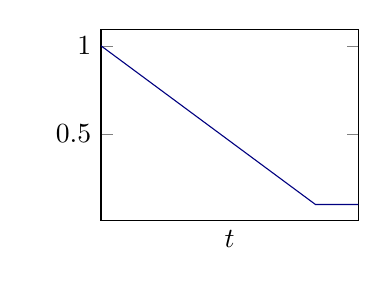
\begin{tikzpicture}
		\begin{axis}[
				xmin=0, xmax=120, width=0.4\textwidth, height=4cm,
				xlabel=$t$, ylabel=\eps{}, xtick=\empty]
			\addplot [blue!50!black] coordinates {
				(0, 1)
				(100, 0.1)
				(120, 0.1)
			};
		\end{axis}
	\end{tikzpicture}
	\qquad
	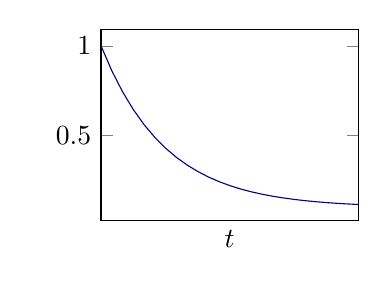
\begin{tikzpicture}
		\begin{axis}[
				xmin=0, xmax=120, width=0.4\textwidth, height=4cm,
				xlabel=$t$, ylabel=\eps{}, xtick=\empty]
			\addplot [blue!50!black, domain=0:120] {
				0.9*exp(-x/30)+0.1
			};
		\end{axis}
	\end{tikzpicture}
	\caption{Probability of a random action over time: \eps{} with linear decay
	(left), \eps{} with exponential decay (right).}
	\label{fig:policy-schedules}
\end{figure}
On the left-hand figure, the probability of a random action is linearly
decreased over time, while on the right, it follows an exponential decay. In
both cases \eps{} never becomes zero, because that would effectively terminate
the learning process. The rate of this decrease is a hyperparameter that
can be tuned.

The most common policies are those just described. They can be directly
used in a RL algorithm or combined to create more complex policies. With
``exploration policy'' we refer to any policy that has a strong component of
nondeterminism and it's suitable to drive the agent's behaviour during
training.


\subsubsection*{Custom exploration policies}

We'll now define few other policies which we proposed and used in this
thesis. Of course, there is no better policy in general. The policies defined
here might be suitable for the environments we face, but may be inappropriate
in many others. They just happen to be useful for one class of environments.

The first one is an $\epsilon$-greedy policy with action repetition. It
chooses between random and deterministic actions just like the
$\epsilon$-greedy. However, consecutive random moves always execute the same
action. This sequence of repetitions can be interrupted by a deterministic
move or by the threshold of maximum repetitions. This policy may be useful in
environments where the effect of a single action is very small. This is the
case, for example, for the exploration of mazes and corridors. The random
policy wouldn't allow the player to cover large distances, because of the
uniform sampling between left and right.

The second policy is an $\epsilon$-greedy with random~$\epsilon$. As we will
see in Section~\ref{sec:training-incremental}, when we need to observe the
environment dynamics, we need to see the observations received in response to
many different stimuli. However, when we apply $\epsilon$-greedy to a capable
agent, we see the following pattern: $\epsilon$ determines the agent's
ability. To a fixed $\epsilon$ corresponds some average ability, and the
cumulative rewards achieved tend to be very similar. Following this intuition,
we define a policy that samples a random $\epsilon$ for each episode.
So, at different episodes, the agent can explore both the early stages and
more distant environment states.

The last policy we define addresses the same problem as the previous one,
producing very diverse trajectories, but in environments with sparse rewards.
When the reward is sparse, we can read it as successful completion of some
sub-task. In this policy, for each episode, we sample a random natural number,
that we call ``checkpoint''. When the number of rewards collected is lower
than the checkpoint, the agent behaves mostly in a deterministic way, because
the purpose is just to proceed. When the number of rewards reaches the
checkpoint number, we act according to a random policy. The idea is to explore
the environment state space at different depths.


\section{Deep Reinforcement Learning}

\label{sec:deep-rl}

Classic RL algorithms, such as SARSA and Q-learning, are tabular methods.
In fact, they store and update the estimate for each pair $(s, a)$
independently. Unfortunately, this requires discrete and small states and
actions spaces. To overcome this very limiting assumption, we need
parametrized value functions and policies.  \emph{Deep Reinforcement Learning}
(Deep RL) is a recent field of RL in which Neural Networks
(NN)\nomenclature{NN}{Neural Network} are used as powerful function
approximators for policies or value functions.

The main advantage of NNs, and parametric models in general, is that they can
be trained in high-dimensional and continuous input spaces. In fact, a good
fit does not require a complete exploration of the input space, which may be
unfeasible or impossible. Instead, they are trained with some form of
Stochastic Gradient Descent on the set of parameters from input-output
samples. Then, the model can be able to generalize to inputs that have been
never observed, in a meaningful way.

Unfortunately, due to approximation and parametrization, Deep RL algorithms
allow very little guarantees about convergence and optimality. Even if the
input space would be explored completely, updates for recent samples would
also affect the regions previously visited. In fact, any effective Deep RL
algorithm introduces some techniques in order to generate a stable training.


\subsection{Popular testbed for Deep RL: Atari games}

\label{sec:atari-envs}

The Atari 2600 is a video game platform that was developed in 1977. There are
hundreds of classic games available to play: Space Invaders, Ms. Pacman,
Breakout and many others. The screen is 160 pixels wide and 210 pixels high,
with RGB colors of 8-bits depth. The joystick has 9 positions (3 for each
axis) and one button, for a total of 18 possible actions. For this reason,
we'll only focus on RL methods for discrete action spaces.

The Arcade Learning Environment~\cite{bib:atari-games} is a simple interface
to the Atari 2600 emulator. It allows agents to play and be trained on these
games. At each step, the agent chooses one of the 18 actions available and
receives in return a frame of the game and a reward. The reward is the
increment in the player's score for the original game. This is really the same
interface that a human player would use. Figure~\ref{fig:atari-frames} shows
the frames from few games in this collection. 

\begin{figure}
	\centering
	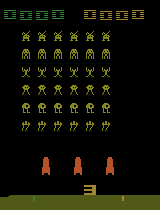
\includegraphics[width=0.25\textwidth]{./imgs/si0.png}
	\quad
	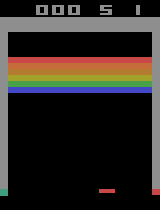
\includegraphics[width=0.25\textwidth]{./imgs/br0.png}
	\quad
	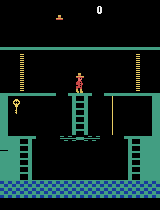
\includegraphics[width=0.25\textwidth]{./imgs/mz0.png}
	\caption{Initial frames of some Atari 2600 games (left to right): Space
		Invaders, Breakout, Montezuma's Revenge.}
	\label{fig:atari-frames}
\end{figure}

Although these games come from an early stage of video games development, they
represent the appropriate challenge for current (Deep) Reinforcement Learning
agents. In fact, many papers tested their RL algorithms on these
games~\cite{bib:atari-deeprl}%
\cite{bib:atari-deepq-nature}\cite{bib:double-q}\cite{bib:rainbow}.
In this thesis, we also tested with some of these environments. We will also
show how improve on the hardest game in this collection for a RL agent:
Montezuma's Revenge.


\subsection{Deep Q-Network}

\label{sec:deep-q-agents}

The \emph{Deep Q-Network} (DQN)\nomenclature{DQN}{Deep Q-Network
algorithm}~\cite{bib:atari-deeprl} was the first algorithm to successfully
combine deep learning models and Reinforcement Learning. Although many basic
ideas presented here have been already introduced by the Neural Fitted
Q~iteration algorithm~\cite{bib:nfq}, DQN addressed some causes of training
instability. They also demonstrated that exactly the same agent can be trained
in many Atari games and achieve human-level performances in many of
those~\cite{bib:atari-deepq-nature}. These promising results sparked a lively
interest in Deep RL, recently.

In DQN, the state-action value is approximated by a deep neural network ${Q(s,
a; \param)}$, on the parmeters $\param$, that we call Q-Network. The purpose
of learning, is to train this network to approximate the optimal q-function: 
$\est{\param}: Q(s, a; \est{\param}) \approx \optimal{q}(s, a)$. Then, the
estimated optimal policy will be:
\begin{equation}
	\est{\policy}(s) = \argmax_{a \in A} Q(s, a; \est{\param})
\end{equation}

A trained network, for each input $(s, a)$, should return the expected value
of some target~$y_{s,a}$. To do so, we select the parameters that minimize the
squared difference between the estimates and the targets:
\begin{equation}
	\text{loss}(\param) \coloneqq \bigl(Q(s, a; \param) - y_{s,a} \bigr)^2
	\label{eq:qnet-generic-loss}
\end{equation}
Since this is a Q-Network, the targets are the optimal state-action
values~$\optimal{q}(s, a)$ that the net should estimate.  The
loss~\eqref{eq:qnet-generic-loss} contains some random variables. So, we
minimize it through any stochastic optimization algorithm. In Stochastic
Gradient Descent (SGD)\nomenclature{SGD}{Stochastic Gradient Descent
algorithm}, at each step $t$, we observe an input ${(s_t, a_t)}$ and the
associated target $y_t$. Then, we take a small step toward the negative
gradient of the loss:
\begin{equation}
	\param_{t+1} = \param_t - \alpha\, \nabla_{\param}\,
	\Bigl( \bigl(Q(s_t, a_t; \param) - y_t \bigr)^2 \Bigr) \Big|_{\param =
	\param_t}
	\label{eq:sgd-update}
\end{equation}
in which $0 < \alpha < 1$ is a small learning rate. This equation is not
the only update rule possible. There are more advanced optimization
algorithms, such as: Momentum, RMSprop and Adam. In this thesis, we've
mostly experimented with Adam.

What has just been described is the usual way of fitting a neural network
to a dataset of samples. In RL, however, the targets $\optimal{q}(s_t, a_t)$
are unknown, because they depend recursively from the same optimal q-function
that we're trying to learn (see equation~\eqref{eq:q-bellman}). In classic RL,
this is not a problem: the 1-step approximation of the q-values (derived from
equation~\eqref{eq:q-bellman}),
\begin{equation}
	y_t \coloneqq r_{t+1} + \discount \max_{a \in A} \est{q}(s_{t+1}, a)
	\label{eq:1step-targets}
\end{equation}
or the n-step approximation, are a valid targets for the function~$\est{q}$.
By updating toward these values on the whole input space, convergence is
guaranteed. In other words, targets can be estimates themselves.

With neural networks, instead, any update to the parameters also affects the
target, because the weights have a global influence on the function. It's not
possible apply a correction for just one tiny region of the input space (nor
it's desirable, after all).  It has been shown~\cite{bib:nfq}, that due to
this effect, propagating errors slow down convergence or even render the
training unstable.  To address this issue one must ensure that the targets do
not move much.

The DQN~\cite{bib:atari-deeprl} algorithm addresses this issue in two ways.
First, the targets in equation~\eqref{eq:1step-targets} are not generated by
the network that is being trained, $Q(s, a; \param)$, but they are computed
from a second net, $Q(s, a; \param')$. Every $C$ iterations, the target net
is updated to match the trained net, with the assignment: $\param' \gets
\param$. This keeps the targets constant for $C$ steps and helps to stabilize
the training.

Second, the network is not trained from the last sample, but from transitions
of the recent experience. At each step, the agent acts according to some
exploration policy, $a_t \sim \policy_e$. Each transition, of the form
$\langle s_t, a_t, r_{t+1}, s_{t+1} \rangle$, is recorded in a buffer of size
$n_r$, called ``experience replay''. Then, at each training step, we sample a
number of $n_b$ transitions, thus creating a batch, and we perform an update
$\param_{i+1} = \param_i - \alpha\, g_i$ on the cumulative gradient $g_i$ of
the whole batch.

DQN also includes a number of heuristics that greatly help the training
but are specific to the Atari~2600 environments:
\begin{itemize}
	\item Rewards can be really high, so they are limited in the range $[-1,
		+1]$; this is called \emph{reward clipping}. It helps to keep the same
		learning rate for diverse games.
	\item The agent has a single life available. When a life is lost, the
		episode ends. This prevents the agent to rely on restarts.
	\item The frames are slightly down-scaled to further reduce the resolution,
		they are transformed to gray-scale and mapped to the range $[-1, +1]$.
		These are common preprocessing steps for NNs.
	\item Every observation is composed by the last 4 frames stacked together.
		This allows the agent to observe how the objects in the scene move.
		See Section~\ref{sec:non-markov} and Example~\vref{ex:motion}.
\end{itemize}

The algorithm used in this thesis is called \emph{Double
DQN}~\cite{bib:double-q}. It is a slight variant of DQN, so all details
mentioned so far also apply. The motivation of this algorithm is a known issue
of Q-learning: it is likely to make overoptimistic value estimates.
To show this, let's rewrite the targets of~\eqref{eq:1step-targets} as:
\begin{equation}
	y_t \coloneqq r_{t+1} + \discount \, Q(s_{t+1}, \argmax_{a \in A} Q(s_{t+1},
	a; \param_t); \param_t)
\end{equation}
where the estimates $\est{q}$ are computed with the Q-Network. This form makes
more evident that the same model is used both to select the next greedy action
and to estimate the q-value of state~$s_t$. As result, any action with an
overestimated q-value will be selected and its value propagated. To remove
this bias, Double DQN decouple the two operations by using different sets of
parameters, $\param\group{1}$ and $\param\group{2}$. The targets $y_t$ are
computed as:
\begin{equation}
	y_t \coloneqq r_{t+1} + \discount \, Q(s_{t+1}, \argmax_{a \in A} Q(s_{t+1},
	a; \param_t\group{1}); \param_t\group{2})
	\label{eq:double-q-targets}
\end{equation}
Then, just the parameters $\param\group{1}$ are updated toward this targets;
this is called the online network. With random chance, the roles of the two
parameters are continuously swapped at each step.

To compute the target, we need to compute the q-values for all actions in
state $s_{t+1}$. To speed up this computation, the network is defined as a
function that takes in input a state and computes a vector of state-action
values, one for each action. So, just one forward pass is required to select
the next action. Common Q-Networks for images are composed of a number of
convolutional layers and some fully-connected layers. The specific structure
may change, and the network used will be defined in the implementation section.

